\section{Mathematical Framework (Numerical Methods)}\label{sec:c5s2}
\lipsum[38-38]

This section builds on the material in \cref{sec:c5s1}, \cref{ch:6} and the prior work of \citet{ch5-9}; see also \citep{ch5-13,ch5-3}.

\begin{equation}\label{eq:c5s2-a}
  \hat{\theta} = \arg\min_{\theta\in\Theta}\; \frac{1}{n}\sum_{i=1}^{n}\ell\bigl(y_i, g_\theta(x_i)\bigr) + \lambda\lVert\theta\rVert_2^2 .
\end{equation}
Under standard regularity conditions the estimator is consistent, and its error satisfies
\begin{equation}\label{eq:c5s2-b}
  \mathbb{E}\lVert\hat\theta-\theta^\star\rVert^2 \le \frac{C\,\sigma^2 d}{n} + \lambda^2\lVert\theta^\star\rVert^2 .
\end{equation}

Equations~\eqref{eq:c5s2-a} and~\eqref{eq:c5s2-b} are used throughout the remainder of this section.

\lipsum[27-28]

\subsection{Quantitative behaviour}\label{sec:c5s2-q}
Results are collected in \cref{tab:c5s2} and visualised in \cref{fig:c5s2-f1}. Similar trends were reported in~\citep{ch5-4,ch5-11}.

\begin{table}[htbp]
\centering
\caption{Summary of measured quantities for experiment set \texttt{c5s2}.}\label{tab:c5s2}
\begin{tabular}{lrrr}
\toprule
Method & Score & Latency & Error \\
\midrule
Alpha & \num{76.5} & \SI{2.74}{\milli\second} & \num{2.610e-2} \\
Beta & \num{85.4} & \SI{6.46}{\milli\second} & \num{1.159e-4} \\
Gamma & \num{98.7} & \SI{5.60}{\milli\second} & \num{5.315e-2} \\
Delta & \num{99.9} & \SI{1.35}{\milli\second} & \num{7.994e-5} \\
Epsilon & \num{31.2} & \SI{3.72}{\milli\second} & \num{2.439e-3} \\
\bottomrule
\end{tabular}
\end{table}

\begin{figure}[htbp]
\centering
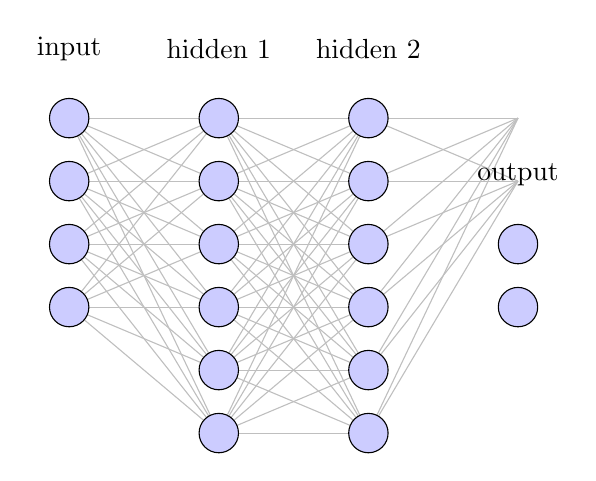
\begin{tikzpicture}[x=1.9cm,y=0.8cm,neuron/.style={circle,draw,fill=blue!20,minimum size=5mm,inner sep=0}]
\foreach \i in {1,...,4}{\foreach \j in {1,...,6}{\draw[gray!50](0,-\i)--(1,-\j);}}
\foreach \i in {1,...,6}{\foreach \j in {1,...,6}{\draw[gray!50](1,-\i)--(2,-\j);}}
\foreach \i in {1,...,6}{\foreach \j in {1,...,2}{\draw[gray!50](2,-\i)--(3,-\j);}}
\foreach \i in {1,...,4}\node[neuron](i\i)at(0,-\i){};
\foreach \i in {1,...,6}\node[neuron](h\i)at(1,-\i){};
\foreach \i in {1,...,6}\node[neuron](g\i)at(2,-\i){};
\foreach \i in {1,...,2}\node[neuron](o\i)at(3,-\i-2){};
\node at(0,0.1){input};\node at(1,0.1){hidden 1};\node at(2,0.1){hidden 2};\node at(3,-1.9){output};
\end{tikzpicture}
\caption{Generated figure for \texttt{c5s2-f1} (parameters $a=2$, $b=8$).}\label{fig:c5s2-f1}
\end{figure}

\lipsum[130-131]

\subsection{Implementation notes}\label{sec:c5s2-i}
The core routine is shown in \cref{lst:c5s2}; its complexity is $\mathcal{O}(N\log N)$ per iteration~\cite{ch5-6}.

\begin{lstlisting}[language=c,caption={Reference implementation for c5s2.},label={lst:c5s2}]
#include <stdio.h>

/* Compute a dot product of two vectors. */
double dot(const double *a, const double *b, int n) {
    double s = 0.0;
    for (int i = 0; i < n; ++i)
        s += a[i] * b[i];
    return s;
}
\end{lstlisting}

\lipsum[132-132]
\begin{theorem}\label{thm:c5s2}
Let $A\in\mathbb{R}^{n\times n}$ be symmetric positive definite with condition number $\kappa$. Then the iteration converges and
$\lVert e_k\rVert_A \le 2\bigl(\tfrac{\sqrt\kappa-1}{\sqrt\kappa+1}\bigr)^k\lVert e_0\rVert_A$.
\end{theorem}
\begin{enumerate}[label=(\roman*)]
\item the bound in \cref{thm:c5s2} is sharp for some initial errors;
\item the constant $2$ cannot be improved in general;
\item preconditioning reduces the effective $\kappa$.
\end{enumerate}

\lipsum[70-70]
